\documentclass{article}

% if you need to pass options to natbib, use, e.g.:
% \PassOptionsToPackage{numbers, compress}{natbib}
% before loading nips_2016
%
% to avoid loading the natbib package, add option nonatbib
% \usepackage[nonatbib]{nips_2016}

\usepackage{nips_2016}

% to compile a camera-ready version, add the [final] option, e.g.:
%\usepackage[final]{nips_2016}


\usepackage[english, status=draft]{fixme} % these 2 make fixme comments :) 
\fxusetheme{color}                        %

\usepackage[utf8]{inputenc} % allow utf-8 input
\usepackage[T1]{fontenc}    % use 8-bit T1 fonts
\usepackage{hyperref}       % hyperlinks
\usepackage{url}            % simple URL typesetting
\usepackage{booktabs}       % professional-quality tables
\usepackage{amsfonts}       % blackboard math symbols
\usepackage{nicefrac}       % compact symbols for 1/2, etc.
\usepackage{microtype}      % microtypography
\usepackage{graphicx}       %PICTSCHA
\usepackage{amsmath}        %METH, ok appears to be included in the amsfontz





%%%%%%%%%%
% citation stuff
%%%%%%%%

\usepackage{natbib} 
%bibstyle muss einer da sein, 
% setimmt wie der kram an \cite aussieht.
% https://de.wikibooks.org/wiki/LaTeX-W%C3%B6rterbuch:_bibliographystyle
%https://de.sharelatex.com/learn/Bibtex_bibliography_styles
%\bibliographystyle{abbrvnat} 
%\bibliographystyle{unsrt} 
\bibliographystyle{plainnat}









\title{A constructive approach for graphs\\with long range dependencies}

% The \author macro works with any number of authors. There are two
% commands used to separate the names and addresses of multiple
% authors: \And and \AND.
%
% Using \And between authors leaves it to LaTeX to determine where to
% break the lines. Using \AND forces a line break at that point. So,
% if LaTeX puts 3 of 4 authors names on the first line, and the last
% on the second line, try using \AND instead of \And before the third
% author name.

\author{
  Fabrizio Costa \\
  Department of Computer Science\\
  Albert-Ludwigs University Freiburg\\
  Freiburg, 79085  \\
  \texttt{costa@informatik.uni-freiburg.de} \\
  \And
  Stefan Mautner\\
  Department of Computer Science\\
  Albert-Ludwigs University Freiburg\\
  Freiburg, 79085  \\
  \texttt{mautner@cs.uni-freiburg.de} \\
  %% examples of more authors
  %%\AND
  %% Coauthor \\
  %% Affiliation \\
  %% Address \\
  %% \texttt{email} \\
  %% \And
  %% Coauthor \\
  %% Affiliation \\
  %% Address \\
  %% \texttt{email} \\
  %% \And
  %% Coauthor \\
  %% Affiliation \\
  %% Address \\
  %% \texttt{email} \\
}

\begin{document}
% \nipsfinalcopy is no longer used

\maketitle

\begin{abstract}
%Scripts describing the generation of generic graphs based on examples
%are scarce.

Machine learning constructive approaches offer a way to answer interesting
'design' questions on the basis of a collection of examples. Rather than
focusing on the prediction of specific qualities for a given input object,
these methods learn how to synthesize novel instances that share the same
characteristics of a selected sample. In particular, graph constructive
methods are of interest in chemo- and bio-informatics domains where the task
is to synthesize novel molecules with a desired bioactivity. Unfortunately
most molecules exhibit complex dependencies between their different
constituent parts. RNA polymers, for example, self interact, with nucleotides
forming bounds that can typically span the entire length of the sequence.
Since modeling long range dependencies is a difficult problem, we propose an
efficient solution, based on edge contractions and vertex identifications,
that builds on top of a recent constructive approach and we show encouraging
experimental results on a RNA sequence synthesis task.

% Graphs are flexible data structures whose generation 
% is a mostly unexplored problem. As discriminative systems for graphs
% exist, it is feasible to direct a generative process.
% An existing method is implementing Markov Chain Monte Carlo 
% sampling which is altering graphs incrementally.
% Alteration is done with a \emph{graph grammar}, a collection
% of sub graphs, grouped by exchangeability.

% \fxwarning{so the abstract was rewritten, i made sure to explain the contraction}
% By contracting edges in a graph i.e. merging adjacent vertices,
% we obtain a more abstract view on a graph. 
% We use this abstraction to overcome the shortcomings of the original 
% grammar.
% However, the modification is required to be automatically generate. 
% We explore the application of this idea
% on graphs representing RNA secondary structure. 



\end{abstract}
\section{Introduction}

Constructive machine learning addresses the problem of automatically 'build'
or 'design' artifacts given a representative set of examples. The task becomes
particularly challenging in a discrete setting when the solution space is
exponential and direct enumeration approaches become unfeasible. In
\cite{costa16} the problem of generating elements of a structured domain was
framed as the equivalent problem of sampling from a corresponding underlying
probability distribution defined over a (learned) class of structures.
Approaches like {\em rejection sampling} where instances are generated without
enforcing constraints, but are then rejected if violations in the probability
distribution occur, are inefficient as the sampling space almost never yields
valid samples. In order to work with objects that have a non negligible
probability of being accepted they use a context-sensitive graph grammar. The
authors acknowledge that an approach based exclusively on a grammar is not
sufficient to adequately solve the constructive machine learning problem. In
fact, the number of proposed graphs grows exponentially with the number of
production rules in the grammar. In order to select only the most promising
candidates one needs to equip the grammar with a probabilistic notion. However
any procedure to estimate the probabilities of a context-sensitive grammar
needs to trade off the number of contextual rules with the expressiveness of
the grammar. The larger the context, the (exponentially) larger the number of
possible cases that need to be observed for a reliable estimate, which in turn
requires an exponentially large number of training examples. For this reason
global or just long range constraints cannot be effectively modeled, resulting
in a grammar that could express non viable instances. To address the issue in
\cite{costa16} it is proposed to use a Metropolis Hastings (MH) Markov Chain
Monte Carlo (MCMC) method, where the problem of sampling is reduced to the
easier task of {\em simulation}, provided that one can build an ergodic Markov
chain with the desired distribution as its equilibrium distribution. They use
the context sensitive graph grammar to inform the MH proposal distribution,
but also introduce a probability density estimator to define the MH acceptance
procedure. This allows to deal separately with local and global constraints:
the locally context-sensitive graph grammar is used for the local constraints
and the regularized statistical model is used for the global or long range
constraints. The two approaches complement each other: the grammar is a
flexible non-parametric approach that can model complex dependencies between
vertices that are within a short path distance from each other; the
statistical model, instead, can employ the bias derived from the particular
functional family (linear) and the type of regularization used (a penalty over
the L2 norm of the parameters) to generalize long range dependencies to cases
that are similar but not identical to those observed in the training set.

This approach is therefore adequate when natural dependencies exhibit local
constraints that are more complex than long range ones.  Unfortunately in
some application domains instances can exhibit complex long range
dependencies between their different constituent parts. This is the case for
the biological domain where polymers as RNA for example, can be modeled as
long sequences of atomic entities which self interact, establishing pairwise
bounds that can typically span the entire length of the sequence (i.e. non
local interactions).

A different way to view the issue of long range dependencies is that of the
appropriate scale of representation. In certain application domains, instances
are naturally encoded as graphs with nodes that represent atomic entities,
such as nucleotides in the case of RNA sequences. However, it is known that a
more effective functional description of these molecules can be obtained in
terms of structural components such as {\em stems} (stretches of consecutive
paired nucleotides) and {\em loops} (stretches of consecutive unpaired
nucleotides), each made of multiple atomic units. Under this view,
dependencies that are local at the coarser scales correspond to longer range
dependencies at the original scale.

A constructive system suitable for these domains needs to be able to
adequately model complex long range dependencies and is more effective if it
operates at a convenient coarser scale rather than that of the individual
units. Here we tackle all these issues building on the approach presented in
\cite{costa16} introducing two key ideas: 1) we allow a user defined graph
coarsening procedure based on edge contractions and vertex identifications,
and 2) we allow a domain specific optimization approach to ensure that the
generated instances are viable.

%
\begin{figure}[ht]
      \centering
        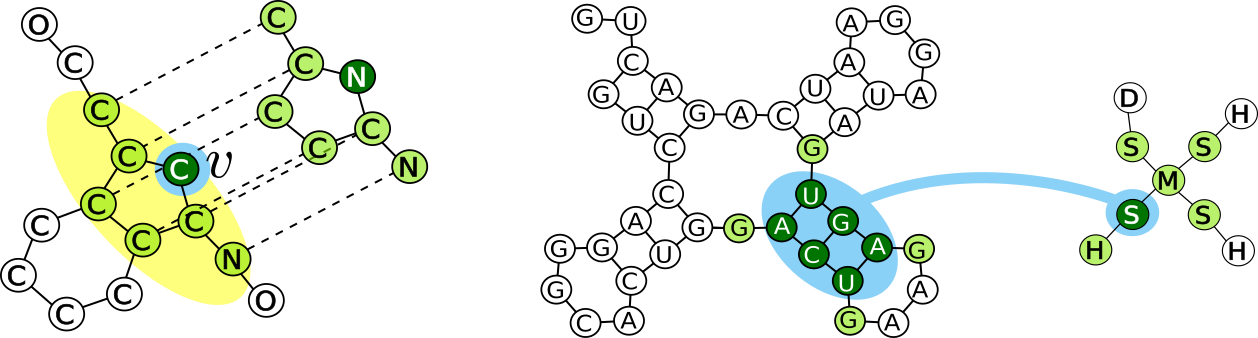
\includegraphics[width=1.0\linewidth]{images/allcipsinone.png}
      \caption{Left: Simplified RNA molecule. Mid: The same molecule
      condensed to its structural elements. Right: Chemical molecule and a
      \emph{congruent} CIP. Core (dark) Interface (brighter) Pair graphs (CIP)
      are
      highlighted in color.}
      \label{allcips}
\end{figure}

\section{Method}

Previously \cite{costa16} introduced a method
to construct novel graphs according to a distribution, which is given by
examples. Graphs are vectorized by a \emph{decomposition kernel}
to train a machine learning model, e.g. an SVM.
Fragments of the graphs are collected in 
a \emph{grammar} (analogous to a string grammar) to alter the initial
set of graphs incrementally. Such changes to a graph are evaluated with the
model. 
We present a method to increase the flexibility of the graph grammar.

\subsection{Previous grammar and definitions}

The grammar consists of sets of interchangeable graph fragments.
We call these fragments core interface pairs(CIPs) because 
they consist of a core part and an interface part.
In terms of a string grammar core and interface are imaginable 
as a production: $iiiCCCiii \Longleftrightarrow iiiCCCCiii$.
In fig. \ref{allcips} (right) we can see a production applied to a graph $G$.
Vertices in \emph{radius} $n$ of a root vertex are the vertices in distance $n$
or less. The (in dark) core area is determined by vertices in a radius $R$
around a root vertex $v$, hence $C_{R}^v(G)$. Here this radius is $0$. In a
lighter green we observe the interface with its Thickness $T$. This is the graph
induced by the vertices in distance $T$ around core vertices, it is
described by $I_{R,T}^v(G)$.


\subsection{contribution}
\textbf{Contraction Extension.}
In place of simple CIPs as used previously,
we use modified CIPs that consider contracted versions
of the original graphs. We obtain a contracted graph $G'$ by contracting edges
in $G$. Fig. \ref{allcips} (mid) is showing the result of multiple contractions
applied to the graph on the left. The set of contracted vertices of a
created vertex is accessible with the $contracted$ function.
The functions for extracting core and interface graphs, 
$C_{R}^v(G')$ and $I_{R,T}^v(G')$, are unaltered except that we apply them
on $G'$ instead of $G$, see fig. \ref{allcips}(mid).
Since the sampling is performed on the uncontracted graphs,
We are now defining related cores and interfaces in $G$.
The core is given by the vertices that were contracted to form $C_{R}^v(G')$.
For the Interface we choose a nodes adjacent to the core in $G$ with a
distance $B$.
The core graph $C_{R}^v(G',G)$ is induced by the nodes 
$\bigcup\limits_{u \in C_R^v(G')} contracted(u)$.
The new interface graph $I_{R,B}^v(G',G)$ is then obtained by the nodes 
$\{ w | d(w,v) \leq B \wedge v\in C_R^v(G',G) \wedge w \in G \wedge w 
\notin C_R^v(G',G) \}$.  $B$ is the thickness of the base graph.
At this point we can construct a CIP from $C_R^v(G',G)$ and $I_{R,B}^v(G',G)$. 
To find a congruent CIP, we previously compared the hashed $I_{R,T}^v(G)$ 
graphs. By combining the hashes of $I_{R,T}^v(G')$ and $I_{R,B}^v(G,G')$ we
increase the specificity of this comparison.
In the intended case $I_{R,T}^v(G')$ (see fig \ref{allcips}(mid)) is small
which means that the
specificity is not increasing too much while still providing
a helpful hint about the context in which a core is seen.
In our application case, we contract according to the
secondary RNA structure and label the resulting vertex accordingly e.g.
'Hairpin loop'.$I_{R,T}^v(G')$  encodes far reaching and abstract
information about the surrounding vertices in our CIP interface matching.


% graph contration, interface trick
% change to congruency
\textbf{An improvement to the notion of congruency.}
CIPs require isomorphism to be considered congruent.
We expand this requirement to incorporate
the distance to the closest nodes in the core graph when 
determining if graphs are congruent.
$\forall u \in I_{R,T}^v(G) : 
\underset{z \in  C_{R}^v(G)}{\min} d(u,z) = 
\underset{z' \in  C_{R}^{v'}(G')}{\min} d(\phi(u),z') $ i.e. the distance 
to the closest core node is equal for every
$u$ and $\phi(u)$.
It is easy to see the benefit of this extension.
Imagine a CIP embedded into a graph. Let the interface consist of
two connected vertices $a$ and $b$, $b$ being adjacent to the core while
$a$ is connected to the rest of the graph.
Clearly a CIP whose $a$ vertex is connected to its core should not be matched.


\textbf{Contracting vertices.}
In this chapter we have seen vertices being contracted
that are connected with an edge. This is not a requirement
as any two vertices in a graph could be contracted. This
is called vertex identification.  
We did so with vertices in the multi-loop that are not stem vertices.
In fig. \ref{allcips} the multi-loop is labeled 'M', the stem 'S'.

\textbf{Adaptation of the sampling process.}
In a sampling step we generate a new graph and decide if
we accept it. The new graph is generated by applying a
production to the current instance. 
In fig. \ref{allcips}(left) we can see an production being applied. 
In the case of the enhanced grammar, the base graph $G$ changes.
These changes may alter the contracted view of the graph.
Therefore the contraction has to be recalculated following each step
of the sampling process.


%\fxwarning{remove this eden part.. what about the directedness? look up what 
%i did!also the hashing part! and then explain it}
%Although the underlying EDeN kernel does not support directed graphs,
%the grammar may contain directed graphs. This is implemented by extracting
%CIPs as if undirected and creating the grammar as usual.
%% need to be able to recalculate abstractions
%A constraint to the contraction is that we need to be able to 
%generate it algorithmically. In the sampling phase we recalculate 
%the contraction after changes to the underlying graph.


\section{Evaluation}
% Infernal is the way to go, also describes secondary structure
RNA sequences are sequences over the four nucleotides A,G,U and C.
The nucleotides are connected to a backbone which 
has a 5' and a 3' end.
Thus, a sequence is translateable into a directed path graph.
Nucleotides may bind to non adjacent nucleotides.
In the graph we introduce a non directed edge between the two nucleotides.
The resulting graph is called the  \emph{secondary structure} graph.
The presented grammar works fine with directed graphs.
RNAs are grouped into functional families whose classification
is a problem of biology. \emph{Infernal}\cite{infernal} can classify and 
create members of these families using covariance models.
Infernal gives us a domain specific way to evaluate
our Method for the generation of new graphs. 


The process of obtaining the secondary structure (graph) for a seqence is 
called folding. Folding is important for RNA to function in a living cell. 
Calculating the physically optimal folding for a single sequence
is possible, but actual sequences will often fold in unison with 
sequences in their family. Therefore, if we are to fold a sequence,
we find the four most similar sequences from the training set and 
look for a consensus structure.
This is done by first aligning the sequences with \emph{muscle} \cite{muscle}
and then folding this alignment with  \emph{RNAalifold}
\cite{rnaalifold}.  

% choose data this way
We chose our RNA sequences from the seed sequences of each family
that Infernal is using\cite{rfam}. Sequences were chosen from RNA families with
a) many members, because some families contain 10
instances which is very few for a classification task. b) interesting 
structure, many sequences fold into structures that exhibit a large number of 
unpaired bases which would result in a very simple contracted graph
c) similar length, because classification should no be trivial.
In the sampling process, many variables are involved. To obtain 
sampling parameters, the parameterspace was randomly searched.
To obtain the grammar parameters, a gridsearch over some options was conducted.



% eval against Infernal
We evaluate our generated sequences with Infernal\cite{infernal}.
For each Familily Infernal provides a model what is trained on 
a hand curated list of familiy representatives as well as a 
bit score threshold. Sequences whose score is above the threshold 
can be considered part of the RNA family. 
Fig. \ref{infeval} shows the average bit-score of generated graphs
and the size of the training set. The black bar represents the threshold.
In blue we see the scores of the sequences generated with the enhanced grammar.
In green the sequences generated by a normal grammar. 
Two results are notiveable 1) the sequences generated by our method
are overwhelmingly above the threshold. 2) the new method outperforms
the old. 

% eval learning curve+ edit dist
Costa \cite{costa14} defines \emph{the constructive learning problem for 
finite samples}.
The goal is to generate graphs that are different from the training set,
but depict a similar distribution.
The similarity of two sets of seqences $a$ and $b$ 
is obtained with $s(a,b)/\sqrt{(s(a,a)*s(b,b))}$ where $s$ is the mean of the
similarity matrix between the two arguments. If the arguments are identical,
the diagonal is removed from the matrix.
Distributions are indirectly comparable by looking at the performance 
of trained estimators. A high similarity in performance indicates a high
similarity in distribution.
Fig \ref{learncurve} shows the average (over positive and negative set)
similarity as described above. 
We also see the learning curves obtained by training an estimator
on $x$ random instances from each of two rna family representatives.
We see the curves for the original seeds, the sequences generated by 
our graph generator and the combined set. 




\begin{figure}[ht]
      \centering
        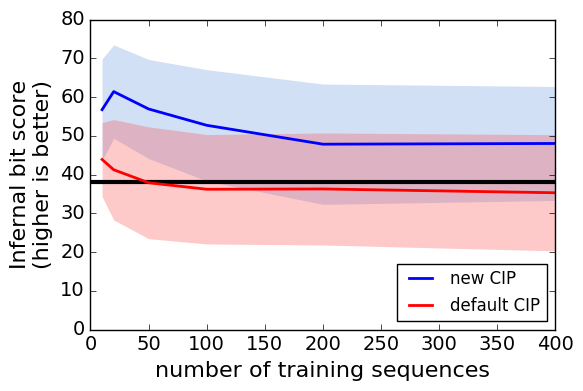
\includegraphics[width=0.5\linewidth]{images/infernal_abstr.png}
      \caption{Infernal evaluation on new method}
      \label{infeval}
\end{figure}
\fxwarning{pictures are not in their final form}

\begin{figure}[ht]
      \centering
        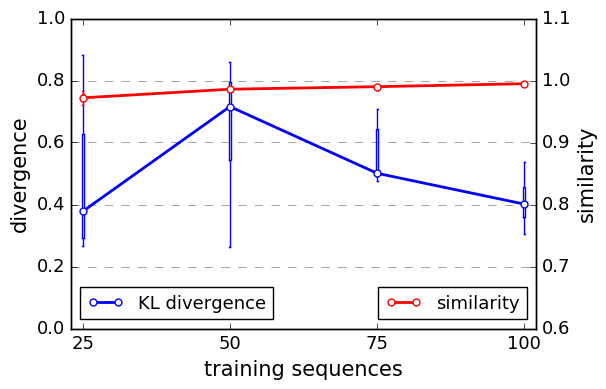
\includegraphics[width=0.5\linewidth]{images/learningcurve.png}
      \caption{learning curve}
      \label{learncurve}
\end{figure}



\section{Discussion and Conclusion}

We have introduced a flexible approach to tackle the problem of long range
dependency modeling for a constructive machine learning approach. Allowing for
a user defined coarsening procedure we have showed how we can synthesize novel
RNA sequences that are functionally equivalent to an original example sample.
The coarsening procedure allows the injection of domain knowledge,
significantly improving the quality of the results over the original domain a-specific approach. In future work we will investigate how to learn task
specific coarsening schemes in a supervised fashion directly from data.


\bibliography{mybib}


\end{document}

